The full mathematical description of the model can be found in [XXX]. The description provided here omits certain details, but is sufficient to understand the inter-process communication that enables distributed simulation. The model is in the class of \textit{cell transmission} models first introduced by Daganzo in XXX. Since then there have been many extensions and improvements to the CTM, incorporating multiple lanes, non-triangular fundamental diagrams, etc. The CTM model that is implemented in OTM is adapted to an underlying representation of the road that is shared among 
all models in the hybrid simulation environment. As with most traffic simulators, there is a high-level graph (links and nodes) which provides the connectivity between roads at intersections. Each link (i.e. a segment of road between two junctions) has an internal geometry consisting of multiple lanes, lane pockets, and possibly a managed lane with access gates (in the case of a freeway link). There can also be sensors and control devices within the link. 

The relations between lanes that enter and exit a junction are defined by \textit{road connections}. A road connection indicates which lanes in an upstream link can turn into which other lanes in a downstream link. For example, a road connection may indicate that vehicles must be in the outer two lanes of the freeway in order to reach the offramp. The road connections the leave a link can be used to group the lanes of the link that travel at similar speeds. These form the \textit{lane groups}; in our previous example, the two outer lanes constitute a lane group, and the remaining inner lanes are another. 

\begin{figure}[h!]
    \centering
    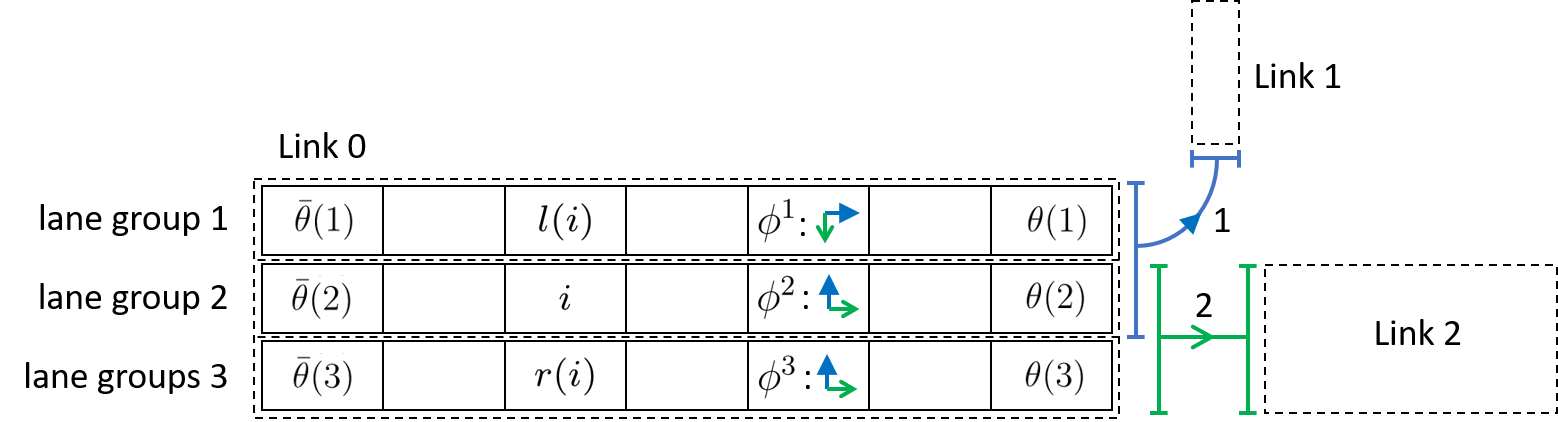
\includegraphics[width=\columnwidth]{figs/cells.png}
    \caption{CAPTION.}
    \label{fig:cells}
\end{figure}

In the CTM model of OTM, each lane group is divided into a sequence of cells, as shown in Figure \ref{fig:cells}. Vehicles are classified according to their \textit{type}. The vehicle type encodes two sets of parameters. First, it determines the vehicle's routing behavior which may be route-based or probabilistic. Route-based vehicles follow a predetermined sequence of links from their origin to their destination. Probabilistically routed vehicles direct themselves at every junction according to time-varying turning probabilities. The software supports arbirary numbers of route-based and probabilistic vehicle types. The second parameter encoded by the vehicle type is the \textit{passenger-vehicle equivalent factor}. This factor scales the size of the vehicle in the calculation of demand. For example a truck may have a passenger-vehicle equivalent factor of 3, meaning that it occupies the space of three passenger vehicles.

The state of each cell is the number of vehicles in the cell for each vehicle type and each downstream link. The downstream link of a vehicle is the next link in its route. This is determined in step XXX below for probabilistically routed vehicle types. Vehicles change lanes (ie move laterally between cells in adjacent lane groups) in order to reach a lane group that connects (via road connections) to its downstream link. 

The state update equation for each cell is executed in the following steps:

\vspace{1em} \noindent \textbf{1) Demand and supply calaculations.} The total demand and supply for every cell are computed using the standard formulas of the cell-transmission model for a triangular fundamental diagram. For the downstream-most cell in each lane group, the demands are referenced to the road connections that connect to the respective downstream links\footnote{OTM imposes the restriction that there can be at most one road connection joining a given upstream lane group to a downstream link}. Prior to computing the longitudinal demand, the model executes all lateral movements (lane changes). [XXX] provides the details. 

\vspace{1em}\noindent \textbf{2) Inter-link flow calculation.} The flows between links travel along road connections. The \textit{node model} resolves these flows from upstream demands and downstream supplies. The details of the node model can be found in XXX. Here it will suffice to state that the output of the node model is a set of \textit{state packets} that are delivered along road connections to downstream links. The node model ensures that the downstream links have sufficient available space to accomodate the state packets.  

\vspace{1em}\noindent \textbf{3) Probabilistic routing.} 
In Figure~\ref{fig:cells}, vehicles that enter link 0 must decide whether they will proceed to link 1 or link 2. This selection is made by probabilistically routed vehicles \textit{upon entering} link 0 by sampling a predifined turning probability distribution. This sampling step is carried out as state packets arrive to a link through a road connection. 

\vspace{1em} \noindent \textbf{4) State update.} Once all packets have been received and tagged with their next downstream link, then the state of the cells can be updated using the conservation of vehicles. This calculation follows the standard cell transmission model formulas for internal cells, and involves the inter-link packets for the first and last cells in a lane group. 

\subsection{Network partitioning}

The first step in the distribution of computation over $n$ processes is to split the network into $n$ overlapping subnetworks. To obtain these, the set of nodes is first partitioned into $n$ non-overlapping sets. Use $\mathcal{N}_i$, $i\in[1\hdots n]$, to denote the $i$th subset of nodes. The $i$th subnetwork contains all of the nodes in $\mathcal{N}_i$, as well as all of the links with either its start or its end node in $\mathcal{N}_i$. 
Links with start node in one subset and end node in another constitute the \textit{overlap} between two subnetworks. An overlap link with start node in $\mathcal{N}_i$ and end node in $\mathcal{N}_j$ is called a \textit{relative source} with respect to subnetwork $j$ and a \textit{relative sink} with respect to subnetwork $i$. The road connections that enter (exit) a relative source (sink) link are called \textit{relative source (sink) road connections} (with respect to a given subnetwork). The implementation includes an off-line module that invokes METIS [XXX] to create the node subsets, and then constructs separate inpute files for each of the subnetworks. These files contain all of the information (and \textit{only} that information) that is required to run the given subnetwork as a stand-alone simulation. 

\subsection{Process communication}

The connections between the $n$ subnetworks are encoded in a \textit{metagraph}. This is a graph in which each vertex represents the non-overlapping portions of a subnetwork, and the edges are the overlapping links. Each subnetwork (internal links as well as overlapping links) is managed by a separate process. The appropriate MPI communicator for this configuration is the 'graph communicator', which encodes the relations of the metagraph. An 'all-to-all' transmission with a graph communicator exchanges messages amongst neighboring vertices in the metagraph. 

The message passed between two neighboring processes consists of an array of numbers representing the vehicles that travel along all of the relative source and sink road connections that join the two subnetworks. During the initialization phase, the processes construct and exchange decoder maps with each of their neighbors. These map each position in the array to a lange group and state index. This same map is used throughout the entire simulation. The approach is conservative in the sense that the size of the message is fixed, and may contain many zeros at any given time. 

The number of vehicles that travel at each time step over road connections (i.e. the flow between links) is computed by the node model in step 2. The MPI communication step is then inserted between steps 2 and 3 from Section XXX. This completes the input and output flow computation for relative sources and sinks. After this, step 3 is executed to compute the downstream link for probabilistically routed vehicles, and then the internal state of all of the lane groups is updated. These steps are identical to their counterparts in the sequential model. Hence the result is not affected by the distribution of the calculation over multiple processes.

\section{A small example}
asdf sadf asdf asdf 


